\documentclass{exam}

\usepackage[dvipsnames]{xcolor}
\usepackage{amsmath}
\usepackage{amsfonts}
\usepackage{amsthm}
\usepackage{microtype}
\usepackage{siunitx}
\DeclareSIUnit\year{yr}
\usepackage{pgfplots}
\usepackage{graphicx}
\usepackage{sidecap}
\sidecaptionvpos{figure}{c}
\usepackage{float}
\usepackage{gensymb}
\usepackage{tkz-euclide}
\usetkzobj{all}
\usepackage{commath}
\usepackage{hyperref}

\newtheorem*{thm}{Theorem}

% russian integral
\usepackage{scalerel}
\DeclareMathOperator*{\rint}{\scalerel*{\rotatebox{17}{$\!\int\!$}}{\int}}

% \qformat{Question \thequestion: \thequestiontitle\hfill}

\begin{document}

\section*{NCEA Level 1 Mathematics (Trigonometry)}

\subsection*{Reading}
\subsection*{Questions}
\begin{questions}

\question Consider two flagpoles a distance \SI{70}{\metre} apart.
          \begin{center}
            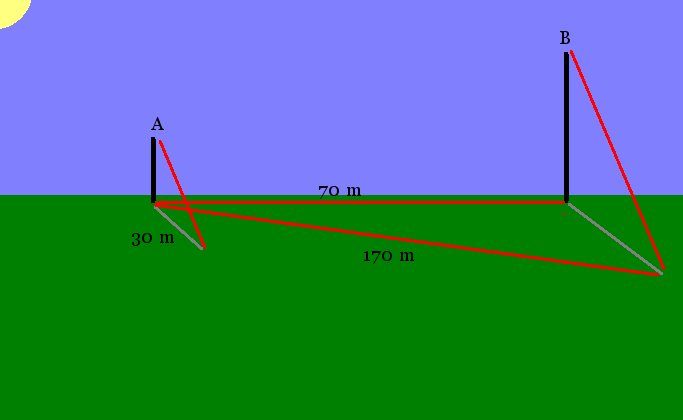
\includegraphics[width=0.5\textwidth]{flagpoles}
          \end{center}
          The angle of the sun above the scene is \SI{30}{\degree}; the shadow of flagpole $ A $ is \SI{30}{\metre} long, and
          the distance from the base of flagpole $ A $ and the end of the shadow of flagpole $ B $ is \SI{170}{\metre}.
  \begin{parts}
    \part Calculate the heights of flagpoles $ A $ and $ B $.
    \part Round your solution to part (a) to the correct number of significant figures; justify your choice.
  \end{parts}

\question In this question, we will prove that for all angles $ x $,
          \begin{displaymath}
            (\sin x)^2 + (\cos x)^2 = 1.
          \end{displaymath}
          In other words, the sum of the two waves in the following diagram is constant.
          \begin{center}
            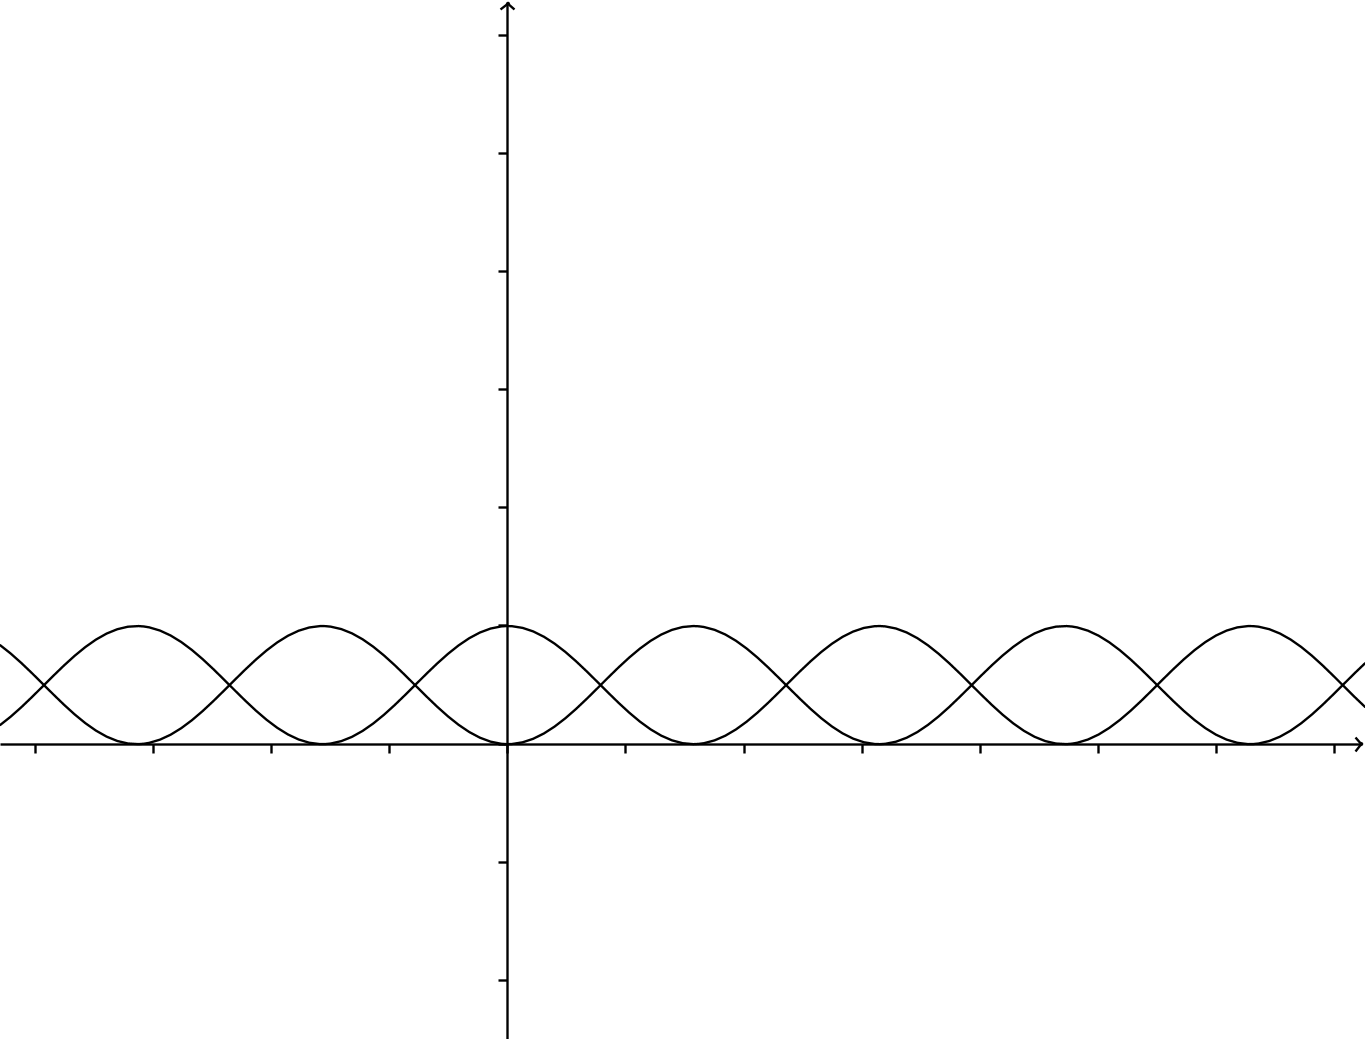
\includegraphics[width=0.5\textwidth]{pythagsine}
          \end{center}
  \begin{parts}
    \part Draw a right angled triangle with hypotenuse 1.
    \part Pick an acute angle and call it $ x $.
    \part Find the lengths of the two non-hypotenuse sides using the trig ratios.
    \part Apply the Pythagorean theorem.
  \end{parts}


\end{questions}
\end{document}
